%%%%%%%%%%%%%%%%%%%%%%%%%%%%%%%%%%%%%%%%%%%%%%%%%%%%%%%%%%%%%%%%%%%%%%%%%
% Some Macro shenanigans to allow for different setups
%%%%%%%%%%%%%%%%%%%%%%%%%%%%%%%%%%%%%%%%%%%%%%%%%%%%%%%%%%%%%%%%%%%%%%%%%
\def\finalsub{final}%
\def\firstsub{first}%
\def\arxivsub{arxiv}%
%\def\submissiontype{first}%   % uncomment this line to output first submission type (if not using bash script/command line);
                               % ONLY UNCOMMENT ONE OF THESE TWO!!
%\def\submissiontype{arxiv}%   % uncomment this line to output arxiv submission type (if not using bash script/command line);
                               % ONLY UNCOMMENT ONE OF THESE TWO!!
\ifx\submissiontype\undefined%
\def\submissiontype{final}%
\fi%
\ifx\submissiontype\firstsub%
\PassOptionsToPackage{twoside}{geometry}
\fi%
\documentclass[titlepage,shield]{hwthesis}
%%%%%%%%%%%%%%%%%%%%%%%%%%%%%%%%%%%%%%%%%%%%%%%%%%%%%%%%%%%%%%%%%%%%%%%%%
% Common packages
%%%%%%%%%%%%%%%%%%%%%%%%%%%%%%%%%%%%%%%%%%%%%%%%%%%%%%%%%%%%%%%%%%%%%%%%%
\usepackage{amsthm,graphicx,subfigure,a4wide,exscale,relsize,setspace,lineno}
\usepackage[square,numbers,sort&compress]{natbib}
\usepackage{geometry}
\usepackage{algorithm2e}
\usepackage[nottoc]{tocbibind}
\usepackage[title,titletoc]{appendix}
\usepackage{tikz} % the one true package for figures
\usetikzlibrary{matrix,cd,arrows} % packages commonly used with tikz
\usepackage{mathtools} % who would not want some mathtools
\usepackage{amsmath,amssymb} % for all the mathematical goodness
\usepackage{tensor}   % more options for indices
\usepackage{mathrsfs} % contains fancy math fonts
\usepackage{bbm}      % contains the double-lined letters used for sets (like N) and fields (like R)
\usepackage{booktabs} % pretty tables, see documentation on how to use
\usepackage{pdfpages} % needed to include researchthesissubmission form
\usepackage{enumitem} % more itemize options
\setlist{nosep}        % enumerate-option which reduces the seperation in itemize list (this looks better
				       % as we already have massive line seperation)
				       
\usepackage{lipsum}    % you can delete this. it just gives a textexample for this template				       

%%%%%%%%%%%%%%%%%%%%%%%%%%%%%%%%%%%%%%%%%%%%%%%%%%%%%%%%%%%%%%%%%%%%%%%%%
% Geometry, hyperref setup and hyperref - dependent on input option
%%%%%%%%%%%%%%%%%%%%%%%%%%%%%%%%%%%%%%%%%%%%%%%%%%%%%%%%%%%%%%%%%%%%%%%%%
\ifx\submissiontype\arxivsub%
\geometry{
 a4paper,
 textwidth = 430 pt,
 textheight = 630 pt
 }
\else%
\geometry{
 a4paper,
 left=40mm,
 right=20mm,
 top=20mm,
 bottom=20mm,
 }
\fi%

% Define linkcolor
\definecolor{MyDarkBlue}{rgb}{0.15,0.25,0.45}

% hyperref setup to have links of appropriate color
\usepackage{hyperref}
\ifx\submissiontype\arxivsub%
\hypersetup{
hypertexnames=false,
colorlinks=true,
citecolor=MyDarkBlue,
linkcolor=MyDarkBlue,
urlcolor=MyDarkBlue,
pdfauthor={John Doe},                     % DO NOT FORGET TO CHANGE AUTHOR,
pdftitle={PhD Thesis of Doom},            % TITLE,
pdfsubject={hep-th math-ph},              % AND SUBJECT!
breaklinks=true
}
\else%
\hypersetup{
hypertexnames=false,
colorlinks=true,
citecolor=black,
linkcolor=black,
urlcolor=black,
pdfauthor={John Doe},                     % DO NOT FORGET TO CHANGE AUTHOR,
pdftitle={PhD Thesis of Doom},            % TITLE,
pdfsubject={hep-th math-ph},              % AND SUBJECT!
breaklinks=true
}
\fi%

\ifx\submissiontype\arxivsub%
\relax
\else%
\linespread{1.5}    % this actually accomplishes one-and-a-half-spacing as required by the guidelines for phd thesis'
\fi%                % the usual command \onehalfspacing uses a weird/its own definition of what one-and-a-half-spacing should mean
                    % the more natural and historical definition is what is accomplished with \linespread{1.5}, similar to what Word
                    % would do. The file size12.clo already defines a space of 14.5pt instead of 12pt and \linespread{1.2414} is
                    % therefore what corresponds to \onehalfspacing, i.e. the lineskip is 1.5 times the lineheight. Word just
                    % multiplies the lineskip 14.5 with another factor of 1.5 more in line with the 'comments should fit inbetween'
                    % requirement.


%%%%%%%%%%%%%%%%%%%%%%%%%%%%%%%%%%%%%%%%%%%%%%%%%%%%%%%%%%%%%%%%%%%%%%%%%
% Macros and Warning suppression
%%%%%%%%%%%%%%%%%%%%%%%%%%%%%%%%%%%%%%%%%%%%%%%%%%%%%%%%%%%%%%%%%%%%%%%%%
\usepackage{macros} % use the macros in macros.sty, optional, edit as convenient; need the abstract-environment inside somewhere however!


\hfuzz=50pt % use this to temporarily turn off overfull warnings to have a better overiew of warnings
\global\hbadness=100000 % use this to temporarily turn off underfull warnings to have a better overview of warnings

% Make the headers in the appendices be "Appendix A: Blah" rather than "Chapter A: Blah".
\let\oldapp\appendix
\renewcommand{\appendix}{\oldapp\renewcommand*{\chaptername}{\appendixname}}

\begin{document}

%%%%%%%%%%%%%%%%%%%%%%%%%%%%%%%%%%%%%%%%%%%%%%%%%%%%%%%%%%%%%%%%%%%%%%%%%
% Make titlepage and top matter
%%%%%%%%%%%%%%%%%%%%%%%%%%%%%%%%%%%%%%%%%%%%%%%%%%%%%%%%%%%%%%%%%%%%%%%%%

\title{PhD Thesis of Doom}

%\subtitle{}

\date{\today} % this gives the current date in MONTH, YEAR format - as required by the guidelines

\author{John Doe} % don't forget do change this to your name

%\address{ $^1$Department of Mathematics and the Maxwell Institute for Mathematical Sciences, Heriot-Watt University, Edinburgh, EH14 4AS, Scotland, UK. }

\maketitle
\pagenumbering{gobble}
\ifx\submissiontype\firstsub%
\mbox{}
\fi%

\begin{abstract}
Abstracting.
\end{abstract}
\ifx\submissiontype\firstsub%
\mbox{}
\fi%

\clearpage
\vspace*{12cm}
\hfil
\hspace{6.5cm}
\textit{To dedicate thesis change these words.}
\clearpage
\ifx\submissiontype\firstsub%
\mbox{}
\clearpage
\fi%

\begin{acknowledgements}
Thanks.
\end{acknowledgements}
\ifx\submissiontype\firstsub%
\mbox{}
\fi%

\ifx\submissiontype\arxivsub%
\relax
\else%
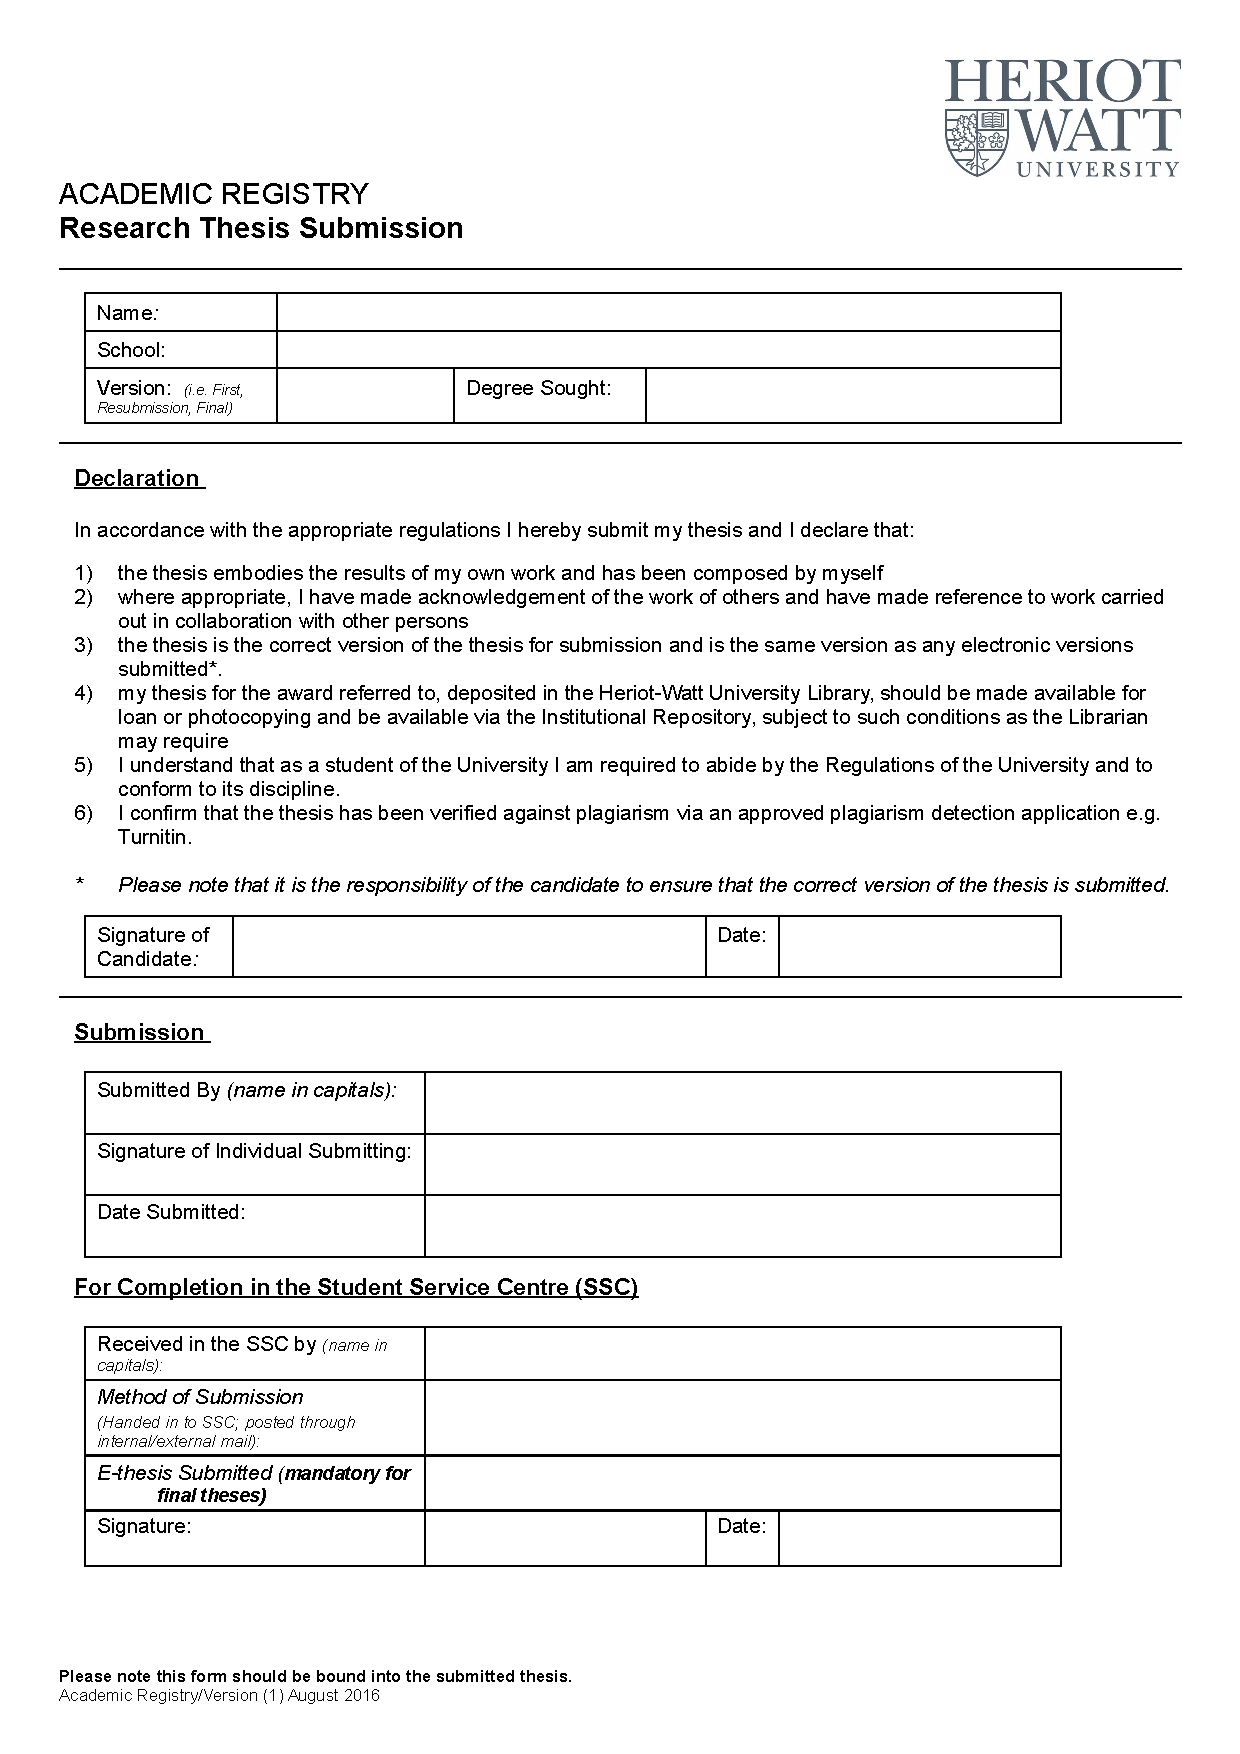
\includepdf[pages={1}]{researchthesissubmission.pdf}
\ifx\submissiontype\firstsub%
\mbox{}
\fi%
\fi%

\clearpage
\setcounter{page}{1}
\pagenumbering{roman}

\tableofcontents
%\listoftables % optional
%\listoffigures % optional

%%%%%%%%%%%%%%%%%%%%%%%%%%%%%%%%%%%%%%%%%%%%%%%%%%%%%%%%%%%%%%%%%%%%%%%%%
% Switch to arabic numbering and input content
%%%%%%%%%%%%%%%%%%%%%%%%%%%%%%%%%%%%%%%%%%%%%%%%%%%%%%%%%%%%%%%%%%%%%%%%%
\clearpage
\pagenumbering{arabic}
\chapter{Introduction}
You need an introduction. This is the first chapter. Above we counted pages in small roman letters. Now we start counting anew using arabic numbers. This is as recommended in the guidelines.
\section{Example Section}
The chapters are split into sections (and subsections if you want). We can cite as normal \cite{Baez:9705009}.

Paragraphs are indented as usual. You can use preset Definition, Theorem and Corallary environments or define your preferred versions yourself.
\begin{mydef}[A Definition]
The current preset looks like this and is counted as $\langle{\rm Chapter Number}\rangle.x$.
\end{mydef}
\begin{mythm}[A Theorem]
Theorems work the same way and count together with definitions.
\end{mythm}
\begin{mycor}[A corollary]
And corollaries count dependent on the last theorem. You can of course change all this as usual --- currently you can find this in \texttt{macros.sty}.
\end{mycor}
\chapter{Example Chapter}
Put as many chapters as you want.

\section{Example Section}
\lipsum
\chapter{Conclusions}
Concluding remarks.

\appendix 
\chapter{Example Appendix}
Appendices work the same way and are labeled with Roman letters.
\section{Example Section}
Same goes for sections.

\bibliography{bigone}  % change this to the name of your bib-file

\bibliographystyle{latexeu}

\clearpage

\end{document}
